%%%%%%%%%%%%%%%%%%%%%%%%%%%%%%%%%%%%%%%%%%%%%%%%%%%%%%%%%%%%%%%%%%%%%%%%%%%%%%%%
%2345678901234567890123456789012345678901234567890123456789012345678901234567890
%        1         2         3         4         5         6         7         8

%\documentclass[final,letterpaper, 10 pt, conference]{ieeeconf}  % Comment this line out if you need a4paper

%\documentclass[10pt, conference, compsocconf]{IEEEtran}
\documentclass[a4paper, 10pt, conference]{ieeeconf}      % Use this line for a4 paper

\IEEEoverridecommandlockouts                              % This command is only needed if
                                                          % you want to use the \thanks command

\newcommand{\eu}{\textrm{e}}
\newcommand{\figref}[1]{Fig.~\ref{fig:#1}}
\overrideIEEEmargins
\usepackage[obeyFinal]{todonotes}
\RequirePackage{graphicx}
\usepackage{subfigure}
\usepackage{bm}
%\usepackage{subequation}
\graphicspath{ {figures/} }
\usepackage{url}
%\usepackage[tight,footnotesize]{subfigure}
\usepackage{fainekos-macros}
\newcommand{\hatodo}[1]{\todo{HA: #1}}
\newcommand{\hatodoin}[1]{\todo[inline]{HA: #1}}
\newcommand{\sAccu}{\epsilon}
\newcommand{\sDelay}{\delta}
\newcommand{\de}{(\sDelay,\sAccu)}
\newcommand{\dek}[1]{(\sDelay_{#1},\sAccu_{#1})}
\newcommand{\hWc}{\widehat{\Wc}}
\newcommand{\sDelayV}{\underline{\sDelay}}
\newcommand{\sAccuV}{\underline{\sAccu}}
\newcommand{\ESet}{\mathcal{E}}
%\newcommand{\bm}{\hat{B}}
\newcommand{\MPCProb}[1]{\mathbb{P_{#1}}}
\newcommand{\RAMPCProb}[2]{\mathbb{P}_{#1}(\hat{\stPt}_{#2},\sDelay_{#2},\sAccu_{#2},\inpPt_{#2 -1})}
\global\long\def\ZSet{\Zc}
\global\long\def\Cc{\mathcal{C}}
\global\long\def\Nom#1{\overline{#1}}
\newcommand{\bla}[1]{\overbar{#1}}
\newcommand{\bli}[1]{\overline{BLI #1}}
%\newboolean{TECH_REPORT}
%\setboolean{TECH_REPORT}{FALSE}
\newcommand{\Given}{|}

\usepackage{array}
\usepackage{url}

%\newcommand\Mark[1]{\textsuperscript#1}


% See the \addtolength command later in the file to balance the column lengths
% on the last page of the document

% The following packages can be found on http:\\www.ctan.org
%\usepackage{graphics} % for pdf, bitmapped graphics files
%\usepackage{epsfig} % for postscript graphics files
%\usepackage{mathptmx} % assumes new font selection scheme installed
%\usepackage{times} % assumes new font selection scheme installed
\usepackage{amsmath} % assumes amsmath package installed
\usepackage{amssymb}  % assumes amsmath package installed
%\begin{document}
\title{\LARGE \bf
Poster Abstract: Co-Design of Anytime Computation and Robust Control
}
%
\author{ Nischal K.N., Paritosh Kelkar, Dhurva Kumar, Yash Vardhan Pant, Houssam Abbas, Joseph Devietti, Rahul Mangharam% <-this % stops a space
\thanks{*This work was supported by STARnet a Semiconductor Research
Corporation program sponsored by MARCO and DARPA, NSF MRI-0923518 and the US Department of Transportation University Transportation Center Program}% <-this % stops a space
\thanks{The Departments of Electrical and Systems Engineering and Computer and Information Sciences, University of Pennsylvania, Philadelphia, U.S.A.
        {\small
        \{yashpant,habbas,kmohta,nghiem,rahulm\}@seas.upenn.edu, devietti@cis.upenn.edu}}%
}


%\author{\IEEEauthorblockN{Yash Vardhan Pant, Houssam Abbas, Kartik Mohta, Rahul Mangharam}
%\IEEEauthorblockA{The Department of Electrical  \\ and Systems Engineering, \\
%University of Pennsylvania, \\
%Philadelphia, U.S.A\\
%yashpant@seas.upenn.edu, kmohta@seas.upenn.edu, \\habbas@seas.upenn.edu, rahulm@seas.upenn.edu}
%\and
%\IEEEauthorblockN{Joseph Devietti}
%\IEEEauthorblockA{The Department of Computer\\  and Information Sciences, \\
%University of Pennsylvania, \\
%Philadelphia, U.S.A\\
%devietti@cis.upenn.edu}
%}




\begin{document}

\maketitle
\thispagestyle{empty}
\pagestyle{empty}

\section{Motivation}
\label{sec:motivation}

Autonomous vehicles promise significant benefits to society, from reduced accident rates to greater mobility for the elderly. 
The biggest challenge in the design of autonomous vehicles comes from the uncertainty of the environment in which they will operate. 
Their control algorithms must be able to cope with driving events that occur on widely ranging time scales. 
For example, relaxed rural driving can accommodate planning actions every few seconds, while imminent collision avoidance requires planning and actuation on the order of a few milliseconds.
Thus `real-time' performance will imply different things depending on the context. 

A second, related, challenge is that the perception algorithms on-board these vehicles (like object detection based on video feed) must handle a very large amount of data, leading to increased power consumption. 
This is especially true for autonomous vehicles (AVs) since they carry multiple sensors (cameras, LIDAR, radars, ultrasound radars, etc) whose data must be processed in real-time to avoid accidents.

As a result of the variability in the environment, the control and perception systems are over-engineered to operate as if the worst-case conditions always hold. 
This results in unnecessarily high power consumption from the computation platform. 
For example, an autonomous research vehicle has two 4KW power inverters dedicated to computation.
Compare this to the average power drawn by the drivetrain of a small electric vehicle, which is 2.4KW, when modeled  in ADVISOR \cite{nreladvisor} going through the Urban Dynamometer Drive Cycle.
(The peak power draw in the same test is 30 KW).
It is also worth noting that over the past few decades, the power consumption of processors has increased by more than double, while battery energy density has only improved by about a quarter \cite{Lahiri}. 

In the current work, we explore the idea of trading-off computation time and power for quality of output, and how this trade-off affects \emph{control performance}.
We start from the observation that the best quality output from the perception algorithm is not always required for the system to achieve the desired control performance.
For example, the control objective might be to follow the center of a driving lane, and control performance is measured by the deviation from that center.
At slow speeds, poor quality of position estimate may be tolerated since it won't lead to excessive deviations from the center.
Therefore we focus on \emph{anytime perception algorithms} that have a pre-defined set of interruption times. 
In general, the earlier the algorithm is interrupted, the worse is the quality of its output. 
On the other hand, that quality may be sufficient for the control algorithm to achieve its goal.

In \cite{RTSS15} we proposed a way in which a standard perception algorithm can be turned into an anytime algorithm via off-line profiling, and thus can offer a time/power/quality trade-off.
We also designed a model predictive controller than can make use of the trade-off offered by the anytime perception algorithm.
To achieve the time/power/quality trade-off, we produced multiple versions of the perception algorithm.
Broadly speaking, a version that ran for longer produced a higher quality output. 

In this work, we turn our attention to achieving the time/power/control performance trade-off \emph{at a fixed level of output quality}, using \emph{platform-level} optimizations.
Even if the output quality of the perception algorithm is fixed, the \emph{speed} at which the output is computed affects control performance: in general, the longer the computation delay, the worse the control performance.
Specifically, we work with an autonomous car $1/10^{th}$ the size of a regular car (Fig. \ref{fig:traxxas}).
\begin{figure}[t]
	\centering
	\includegraphics[scale=0.08]{traxxas.jpg}
	\caption{Traxxas autonomous car with camera.}
		\label{fig:traxxas}
\end{figure}  
It is equipped with a front facing monocular camera and runs the Vanishing Point perception algorithm \cite{VP1}. 
The on-board computation platform has both a CPU and GPU. 
More details of the experimental setup are in Section \ref{sec:experimentalSetup}.
The platform-level optimization divides the Vanishing Point algorithm into components, and decides whether to run each component on the CPU or GPU, and at what frequency.
The assignment to CPU or GPU is not static: every time the algorithm is executed, a different assignment may result, at a different frequency.
The assignment is dictated by the controller: based on off-line profiling of each processor's performance on each component, the controller decides what quality is currently acceptable while minimizing power consumption. 
The profiling is described in more detail in Section \ref{sec:profiling}.
In the present paper, we present initial results of partitioning the Vanishing Point algorithm and running different components on CPU and GPU, and at different frequencies.
We also provide the related power numbers, demonstrating that a meaningful difference in runtime and power consumption exists depending on the assignment and frequency.
In future work, we design a controller to make use of this and other optimizations, and relate the current results to the control algorithm.


\section{Experiment setup}

In this work, we focus on the particular case of autonomous corridor navigation. For this purpose we use the vanishing point algorithm [??] and PID control to maintain heading parallel to the corridor and stay in the middle of it. We implement our algorithm on a $1/10^{th}$ scale car we developed. This section covers the hardware, the algorithm, and the hardware level knobs which affect the performance of the closed loop system and energy consumption of the computation platform.

\subsection{The hardware}

For our experiments, we converted a Radio controlled Traxxas Rally car into an autonomous robot \ref{}[fig], similar to the ones used in \cite{}[MITsertac]. The computation platform is a NVIDIA Jetson TK1. The Jetson has a quad-core ARM Cortex-A15 CPU and a NVIDIA Kepler GPU. This setup allows us to schedule tasks on the CPU or GPU while observing the effect of this on power consumption and timing performance of the algorithm. More details on this are covered in a later section. The Jetson runs Ubuntu for Tegra as the operating system, and the algorithms are implemented using ROS /cite{}[ROS]. The control signals for the drive and steer motor on the platform are generated by a Teensy 3.1 microcontroller which runs a ROS node which converts the continuous output of the control algorithm to the PWM signal which acts as an input to the motor controller on the Traxxas. Finally, the perception algorithm, which is the vanishing point algorithm, gets images from a front facing Point Grey Firefly MV camera which is capable of recording color images at upto a resolution of 752x480 pixels and upto a frame rate of 60 FPS. Additional sensors are also present in the form of a Lidar, optical flow and a 9-dof IMU, but are not used in this study.

\subsection{Vanishing point based corridor navigation}

The Vanishing point algorithm \cite{}[?] has been used extensively in indoor settings for navigation corridors autonomously \cite{}[?][?]. Our experimental setup also relies on the Vanishing point algorithm, implement in OpenCV \cite{}[opencv] to provide feedback to the control algorithm. The vanishing point algorithm outputs the horizontal distance of the vanishing point from the center of the image frame, this feedback is used by the controller to orient the robot such that the distance of the vanishing point from the center of the image frame become zero, i.e. the robot is aligned with the corridor. 

For brevity, we will not explain in detail the workings of the vanishing point algorithm (the interested reader can refer to \cite{}[?]), but will focus on the major computational tasks that comprise the vanishing point algorithm. As shown in figure \ref{}[?], the major computational tasks of the vanishing point algorithm are (sequentially)

\begin{itemize}
\item Blur: A Gaussian blur is applied on the image for de-noising.
\item Edge detection: We use the Canny Edge detector \cite{}[?] to find edges in the image.
\item Hough Transform: In our implementation, the Hough transform is used to detect lines in the image.
\item Random sample consensus (RANSAC): RANSAC is used to find the lines which best describe the parallel lines which represent the sides of the corridor. These lines intersect in the image plane at the Vanishing Point.
\end{itemize}

\subsection{Exploiting hardware level knobs}
With the vanishing point algorithm, we can execute the Blur, the edge detection and the Hough transform on either the CPU or the GPU. RANSAC runs fast enough to not have a signifcant impact on the total execution time, so we do not consider running it on the GPU.
Execution on the GPU results, in general, in a speed-up over the CPU but at a cost of higher power draw from the Jetson. Additionally, on the Jetson, we can control the performance of the CPU and GPU by changing the clock frequencies at which they operate. This gives us multi-dimensional knobs on the hardware level that we can control to trade-off computation speed and power consumption by the Jetson.





\section{Profiling performance and power consumption}

For the perception algorithm, the first stage of our method is profiling the performance (timing and, if available, quality) and power consumption of the computation. 
To do this profiling, we first navigate the robot manually in corridors and log video from the on-board camera at a high frame-rate. 
We run Vanishing point on this video offline and profile it with different scheduling of the three components (Blur, Canny and Hough) on the CPU and GPU, and at different frequencies of both processors (Fig. \ref{fig:vanishing}).

We wrote a custom C-code library to log power measurements from a Tektronix PWS4205 Programmable DC power supply at 100Hz. 
For this we communicate with the power supply over USB using the USB Test and Measurement Class (USB-TMC) communication protocol. 

%In order to profile the timing performance of the Vanishing point algorithm with different schedules for the three tasks we allocate on either the CPU or the GPU, and the different clock frequencies for the CPU and the GPU, we have a script that runs the vanishing point algorithm for all settings offline and logs the update rate in Hz as well as individual execution times of the components and the power consumption. 
Since for an algorithm like Vanishing point there is no well-defined notion of ground truth, we do not have a measure of accuracy of the algorithm. 
Instead, the vanishing point algorithm's update rate is used as a performance measure, since with faster updates the controller can apply input signals to the car faster, resulting in better control performance. 

Figures \ref{fig:diff freq same assignment}, \ref{fig:same freq diff assignment} show the profiling results.
\begin{figure}[t]
\centering
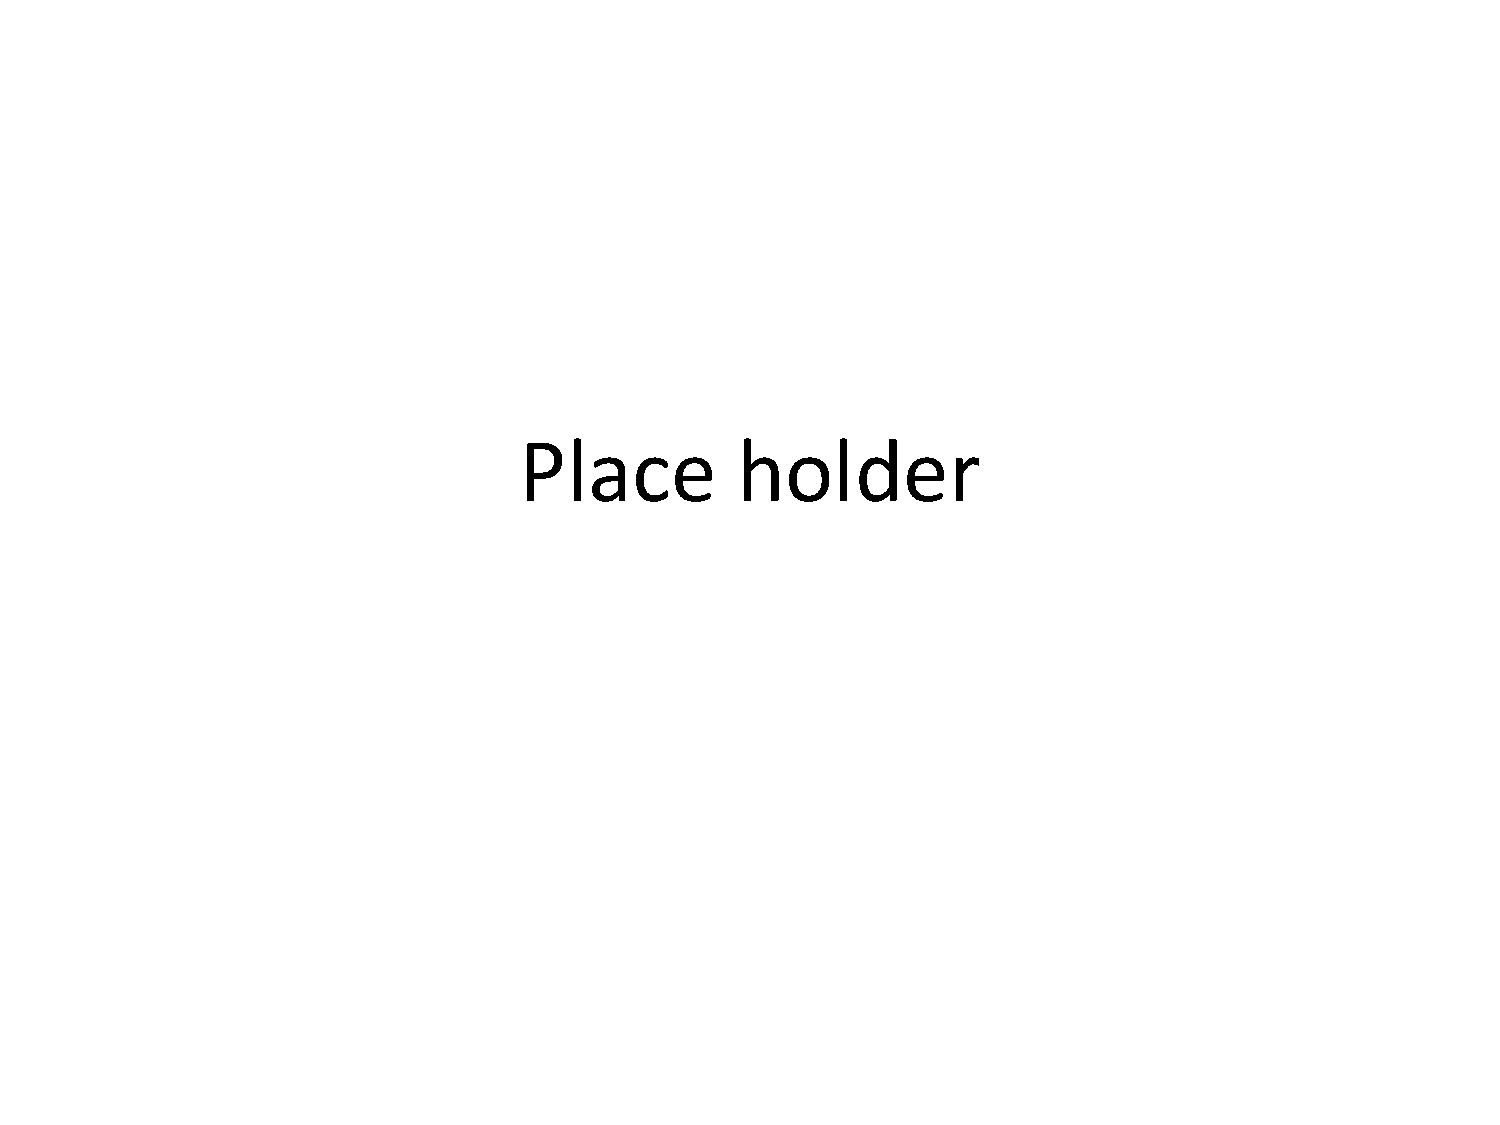
\includegraphics[scale=0.2]{Figs/placeHolder}
\caption{Update rate for different frequencies and a given CPU-GPU assignment.}
\label{fig:diff freq same assignment}
\end{figure}

\begin{figure}[t]
	\centering
	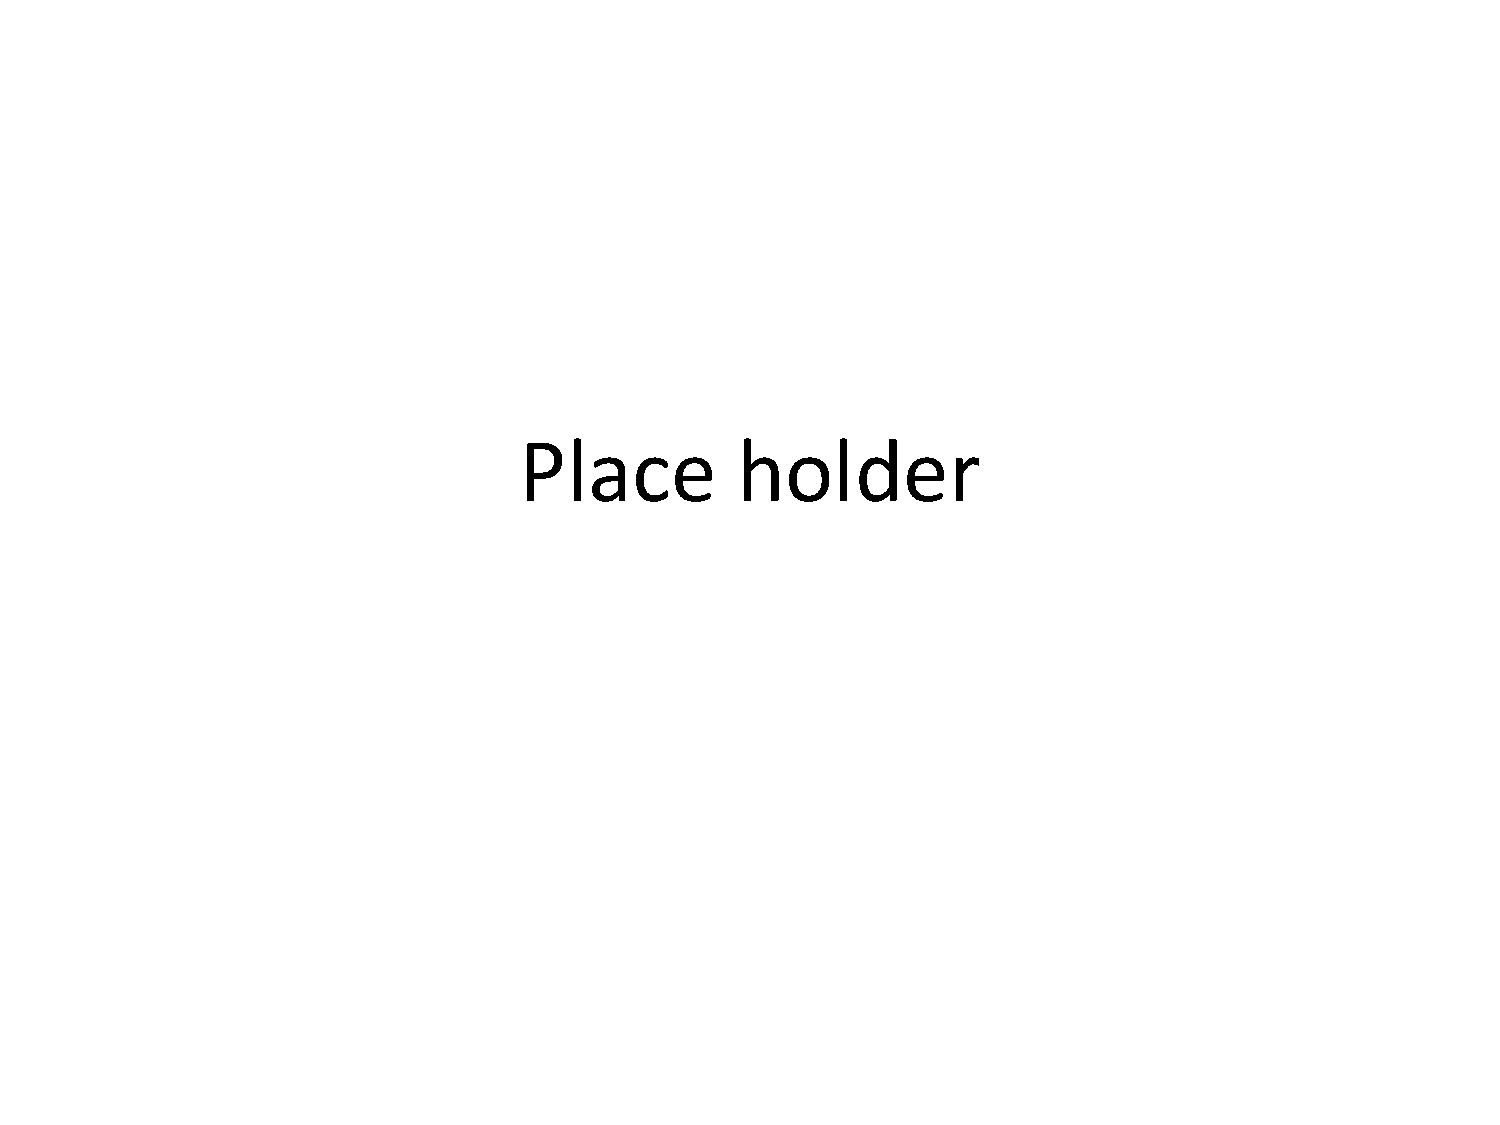
\includegraphics[scale=0.2]{Figs/placeHolder}
	\caption{Update rate for different CPU-GPU assignments at fixed frequencies.}
	\label{fig:same freq diff assignment}
\end{figure}
\section{Future work}

Given the profiling information, on-going work is focused on developing a supervisory algorithm that decides at run-time what mode the perception algorithm should operate in based on the closed loop performance of the system. 
We are also developing a model predictive controller that can leverage the time/power/quality trade-off while guaranteeing safe operation of the closed loop system (e.g., respecting constraints on position and velocity). A more experimental approach also being looked at is switching between multiple PID controllers (each tuned to one mode of the estimation algorithm) based on the error signal from the vanishing point algorithm, which is the only feedback in the simple corridor navigation system which was considered in this work.



%%%%%%%%%%%%%%%%%%%%%%%%%%%%%%%%%%%%%%%%%%%%%%%%%%%%%%%%%%%%%%%%%%%%%%%%%%%%%%%%%
%2345678901234567890123456789012345678901234567890123456789012345678901234567890
%        1         2         3         4         5         6         7         8

%\documentclass[final,letterpaper, 10 pt, conference]{ieeeconf}  % Comment this line out if you need a4paper

\documentclass[10pt, conference, compsocconf]{IEEEtran}
%\documentclass[a4paper, 10pt, conference]{ieeeconf}      % Use this line for a4 paper

%\IEEEoverridecommandlockouts                              % This command is only needed if
% you want to use the \thanks command

\newcommand{\eu}{\textrm{e}}
\newcommand{\figref}[1]{Fig.~\ref{fig:#1}}
%\overrideIEEEmargins
\usepackage[obeyFinal]{todonotes}
\RequirePackage{graphicx}
\usepackage{subfigure}
\usepackage{bm}
%\usepackage{subequation}
\graphicspath{ {Figs/} }
\usepackage{url}
%\usepackage[tight,footnotesize]{subfigure}
\usepackage{fainekos-macros}
\newcommand{\sAccu}{\epsilon}
\newcommand{\sDelay}{\delta}
\newcommand{\de}{(\sDelay,\sAccu)}
\newcommand{\dek}[1]{(\sDelay_{#1},\sAccu_{#1})}
\newcommand{\hWc}{\widehat{\Wc}}
\newcommand{\sDelayV}{\underline{\sDelay}}
\newcommand{\sAccuV}{\underline{\sAccu}}
\newcommand{\ESet}{\mathcal{E}}
%\newcommand{\bm}{\hat{B}}
\newcommand{\MPCProb}[1]{\mathbb{P_{#1}}}
\newcommand{\RAMPCProb}[2]{\mathbb{P}_{#1}(\hat{\stPt}_{#2},\sDelay_{#2},\sAccu_{#2},\inpPt_{#2 -1})}
\global\long\def\ZSet{\Zc}
\global\long\def\Cc{\mathcal{C}}
\global\long\def\Nom#1{\overline{#1}}
\newcommand{\bla}[1]{\overbar{#1}}
\newcommand{\bli}[1]{\overline{BLI #1}}

\usepackage{array}
\usepackage{url}


% See the \addtolength command later in the file to balance the column lengths
% on the last page of the document
\usepackage{amsmath} % assumes amsmath package installed
\usepackage{amssymb}  % assumes amsmath package installed
\renewcommand{\thefigure}{\arabic{figure}}
\title{\LARGE \bf
	Poster Abstract: Hardware optimizations for anytime perception and control
}


\author{\IEEEauthorblockN{Nischal K.N.$^1$, Paritosh Kelkar$^1$, Dhruva Kumar$^1$, Yash Vardhan Pant$^1$, \\
Houssam Abbas$^1$, Joseph Devietti$^2$, Rahul Mangharam$^1$}
\IEEEauthorblockA{$^1$The Department of Electrical and Systems Engineering, \\
$^2$ The Department of Computer and Information Sciences
University of Pennsylvania, \\
Philadelphia, U.S.A\\}
%{nischal,paritosh,dhruvak,yashpant,habbas,rahulm\}@seas.upenn.edu
%yashpant@seas.upenn.edu, \\habbas@seas.upenn.edu, rahulm@seas.upenn.edu}
%\and
%\IEEEauthorblockN{Joseph Devietti}
%\IEEEauthorblockA{The Department of Computer\\  and Information Sciences, \\
%University of Pennsylvania, \\
%Philadelphia, U.S.A\\
%devietti@cis.upenn.edu}
}







%\author{ Nischal K.N., Paritosh Kelkar, Dhruva Kumar, Yash Vardhan Pant, Houssam Abbas\\
%	Joseph Devietti, Rahul Mangharam% <-this % stops a space
%	\thanks{*This work was supported by STARnet a Semiconductor Research
%		Corporation program sponsored by MARCO and DARPA, NSF MRI-0923518 and the US Department of Transportation University Transportation Center Program}% <-this % stops a space
%	\thanks{The Departments of Electrical and Systems Engineering and Computer and Information Sciences, University of Pennsylvania, Philadelphia, U.S.A.
		{\small
%			 \{nischal,paritosh,dhruvak,yashpant,habbas,rahulm\}@seas.upenn.edu, %devietti@cis.upenn.edu}}%
%}


\begin{document}
	
\maketitle
\thispagestyle{empty}
\pagestyle{empty}

In recent years, the development of autonomous vehicles (AVs) has become a major component of the roadmaps of most large automotive manufacturers. 
The perception and control software of these systems have stringent real-time requirements that have to be met for their safe and correct operation.
The uncertain environment in which the AV operates and its complete reliance on sensor data leads to over-engineering, where the system is designed to operate as if the worst-case conditions always hold.
This leads to unnecessarily high power consumption, especially when we consider the large amount of data produced and processed in an AV (from on-board cameras, LIDAR, radars, ultrasonic sensors, high precision GPS, etc). 

In this poster, we present early results of our experiments on a $1/10^{th}$ scale autonomous car. 
The objective of the experiments is to obtain more energy-efficient computations for the perception and estimation algorithms used in autonomous systems by exploiting hardware-level knobs. 
These knobs allow us to leverage a trade-off between computation time, power consumption and output quality of the perception and estimation algorithms. 
In this case, we use a Vanishing Point algorithm to navigate a corridor. 
Vanishing Point is decomposed into three sequential components, and we study how its runtime and power consumption are affected by whether each component is run on a GPU or CPU, and the frequency at which it is executed.
Results highlight CPU/GPU allocation and execution frequencies which achieve better throughput or better power.

Our general method is concerned with how these time/power/quality trade-offs affect control performance. 
We seek to design controllers that can leverage this trade-off to maintain control performance at a lower power cost, or react to a very dynamic driving situation intelligently by obtaining lower quality but more timely estimates of the system's state.   
In the case of the Vanishing Point algorithm, for example, the controller decides at run-time, and for each time step, whether to schedule each of the algorithms's components on the CPU or GPU and at what frequency, to achieve control performance at minimal power. The possible set of operating points and their effect on the update rate and power consumption for the vanishing point algorithm are shown in Figs. \ref{fig:sfda},\ref{fig:sfda_pow}. For each of the three tasks we consider, C (G) represents execution on the CPU (GPU). We can see that a single operating point does not always achieve best overall performance for both update rate and power consumption.
%Ongoing work is focussed on using this profile at run-time and closing the loop with feedback control while selecting operating points for vanishing point on the fly.

\begin{figure}[htbp]
	\centering
	\includegraphics[width=0.46\textwidth]{Data/figs/surf_Rate.pdf}
	\caption{Control update rate for different CPU-GPU assignments at varying frequencies (color in online version).}
	\label{fig:sfda}%same freq diff assignment}
\end{figure}
	%\bibliographystyle{IEEEtran}%abbrv}
	%\bibliography{IEEEabrv,rtss2015,cdc14,anytime_ref,rtss_wip_ref}


\begin{figure}[htbp]
	\centering
	\includegraphics[width=0.46\textwidth]{Data/figs/surf_Power.pdf}
	\caption{Mean power consumed by the vanishing point algorithm (running on the Nvidia Jetson) for different CPU-GPU assignments at varying frequencies. (Color in online version).}
	\label{fig:sfda_pow}%same freq diff assignment}
\end{figure}



\section*{Acknowledgments}
This work was supported by STARnet a Semiconductor Research Corporation program sponsored by MARCO and DARPA, NSF MRI-0923518 and the US Department of Transportation University Transportation Center Program. 
	
\end{document}

%

\bibliographystyle{IEEEtran}%abbrv}
	\bibliography{IEEEabrv,rtss2015,cdc14,anytime_ref,rtss_wip_ref}

	%\section*{Appendix}

\subsection{Constraints of successive MPC problems}
\label{sec:inclusions statement}
We are now ready to state and prove a key lemma regarding the evolution of the state, error and input sets between MPC optimization problems. 
This lemma will be key to proving recursive feasibility of the MPC controller, since it allows us to show that the constraint sets of one problem, at time $k$, are appropriate supersets of the constraint sets of the next problem, at time $k+1$. 

\begin{lemma}
	\label{lem:set inclusions}
	Let $\oa{X}_{k+j|k}$ be the $j$-step outer-approximate reach set computed at time $k$ by a reachability tool as described in Sec. \ref{sec:x reach}.
	
	Let $\What_{k+j|k}$ be the set defined in \eqref{eq:What}.
	
	Let $\tE_{k+j|k}$ be the error set computed using \eqref{eq:H}, \eqref{eq:tildeE} by substituting $E \leftarrow \tE_{k|k}$.
	
	Let $\ua{V}_{k+j|k} = \ua{V}(\oa{X}_{k+j|k})$ and $\oa{V}_{k+j|k} = \oa{V}(\oa{X}_{k+j|k})$ 

Then the following hold for all $k \geq 0, ,j \geq 1$:
\begin{enumerate}
	\item $\oa{X}_{k+1+j|k+1} \subseteq \oa{X}_{k+j+1|k}$
	\label{set:X}
	\item $\tE_{k+1+j|k+1} \subseteq \tE_{k+j+1|k}$
	\label{set:tE}
	\item $\What_{k+1+j|k+1} \subseteq \What_{k+j+1|k}$
	\label{set:What}
	\item $\oa{V}_{k+1+j|k+1} \subseteq \oa{V}_{k+j+1|k}$
	\label{set:oaV}
	\item $\ua{V}_{k+1+j|k+1} \supseteq \ua{V}_{k+j+1|k}$ (note the change in inclusion direction)
	\label{set:uaV}		
\end{enumerate} 
\end{lemma} 

\begin{proof}
	
\ref{set:X}) 
Fix an arbitrary $k$. We prove this by induction on $j \geq 1$.

\underline{Base case: $j=1$}. By construction, $\hx_{k+1} \in \RT{\Xset{k}{k}} \oplus E$.
Therefore at time $k+1$, when setting up the problem $\mathbb{P}_{k+1}(\hat{z}_{k+1})$, the algorithm will first compute
$\Xset{k+1}{k+1} = \hx_{k+1} \oplus (-E)  \subset \RT{\Xset{k}{k}} \oplus E \oplus (-E) = \oaXset{k+1}{k}$.
Also 
$\oaXset{k+2}{k+1} = \RT{\Xset{k+1}{k+1}} \oplus E \oplus(-E) \subset  \RT{\oaXset{k+1}{k}} \oplus E \oplus(-E) = \oaXset{k+2}{k}$.

\underline{Induction step: $j > 1$}.
By definition, $\oaXset{k+1+j}{k+1} = \RT{\oaXset{k+1+j-1}{k+1}} \oplus E \oplus (-E) \subset  \RT{\oaXset{k+j}{k}} \oplus E \oplus (-E)$ (by the induction hypothesis). This last set equals $\oaXset{k+j+1}{k}$ by definition.

\ref{set:tE}) 	By \ref{set:X}) 
 we have that 
 $ \min_{x \in \oa{X}_{k+j+1|k}, e \in E} M_{i\ell}(x)e(\ell) \leq \min_{x \in \oa{X}_{k+1+j|k+1}, e \in E} M_{i\ell}(x)e(\ell)$ and that 
 $\max_{x \in \oa{X}_{k+j+1|k}, e \in E} M_{i\ell}(x)e(\ell) \leq \max_{x \in \oa{X}_{k+1+j|k+1}, e \in E} M_{i\ell}(x)e(\ell)$
 which yields the desired result.
 
 \ref{set:What}) This is immediate from the definition \eqref{eq:What} and \ref{set:tE}).
 
 \ref{set:oaV}) and \ref{set:uaV}) These are immediate from \eqref{eq:V inclusions}.
 
	\end{proof}


\subsection{Proof of Theorem \ref{th:robust_feas}}
\label{sec:proof of thm 1}
We will prove the Theorem by recursion by showing that if at time step $k$, the problem $\mathbb{P}_{k}(\hat{z}_k)$ is feasible and the feasible control input $v_k = v^{*}_{k|k}$ is applied, then $v_k$ is admissible (meets the system constraints) and at time $k+1$, $z_{k+1}$ is inside $Z$ and also $\mathbb{P}_{k+1}(\hat{z}_{k+1})$ is feasible for all disturbances. By recursion then, if we have feasibility at step $k=k_0$, we have robust constraint satisfaction and feasibility at time step $k_0+1$ and so on for all $k>k_0$. 

To begin, let $\mathbb{P}_{k}(\hat{z}_k)$ be feasible, then it has a feasible solution $(\lbrace z^{*}_{k+j|k}\rbrace_{j=0}^{N+1}, \, \lbrace v^{*}_{k+j|k}\rbrace_{j=0}^{N} )$ that satisfies all the constraints of the Robust MPC. 
Now let's construct a feasible candidate solution for $\mathbb{P}_{k+1}(\hat{z}_{k+1})$ at the next time step by shifting the above solution one-step forward. 
Consider the candidate solution:

\begin{subequations}
\begin{align}
\label{eq:candidate}
\nz_{k+j+1|k+1} &= z^{*}_{k+j+1|k} + L_j\hat{w}_{k+1}, \, \forall j \in [0:N]\\
\nz_{k+N+2|k+1}&= A\nz_{k+N+1|k+1} + B\bar{v}_{k+N+1|k+1} \\
\bar{v}_{k+j+1|k+1}&=v^{*}_{k+j+1|k} + KL_j\hat{w}_{k+1}, \, \forall j \in [0:N-1]\\
\bar{v}_{k+N+1|k+1}&=K\nz_{k+N+1|k+1} 
\end{align}
\end{subequations}

First we will show that the input and state constraints are satisfied by $v_k$ and $\nz_{k+1}$, then prove feasibility of the above candidate solution for $\mathbb{P}_{k+1}(\hat{z}_{k+1})$.

\textit{Validity of input and next state:}
The next state is:
\begin{eqnarray}
\label{eq:z_next}
z_{k+1} &= &Az_k + Bv_k + w_k \nonumber
\\
&=& A(\hat{z}_k-\tilde{e}_k)+Bv^{*}_{k|k}+w_k \nonumber \\
 &=& A\hat{z}_k+Bv^{*}_{k|k}-\tilde{e}_{k+1}+(w_k+\tilde{e}_{k+1}-A\tilde{e}_k) \nonumber \\
  &=& Az^{*}_{k|k} +Bv^{*}_{k|k}-\tilde{e}_{k+1}+  \hw_{k+1} \nonumber\\
  & \;& \quad (\Pk{k} \text{ initialization}) \nonumber \\
&= &z^{*}_{k+1|k} - \tilde{e}_{k+1} + \hat{w}_{k+1} 
\end{eqnarray}

By feasibility of the solution at time $k$,
\begin{equation*}
z^{*}_{k+1|k} \in\nomZset{k+1}{k} = Z \ominus (-\tilde{E}_{k+1|k}) \ominus L_0\What_{k+1|k}
\end{equation*}

Therefore, $z_{k+1} \in Z$ and so $x_{k+1} \in X$.
%By definition, $\tilde{e}_{k+1} \in \tilde{E}_{k+1|k}$ and $\hat{w}_{k+1} \in  \What_{k+1|k}$. Using this fact, definition of Pontraygin difference and Eq. \ref{eq:z_next} (also remember, $L_0 = \mathbb{I}$), we have that:

Moreover, by the feasibility of $v^{*}_{k|k}$ for $\mathbb{P}_{k}(\hat{z}_k)$ and by the definition of $\underline{V}_{k|k}$,
$v_k = v^{*}_{k|k} \in \underline{V}_{k|k}$, which implies that $u_k \in U$.

Hence, if $\mathbb{P}_{k}(\hat{z}_k)$ is feasible, then the applied input at time step $k$ and the resulting next state $z_{k+1}$ (and hence $x_{k+1}$) are admissible under all possible disturbances. 
The next part of the proof will focus on showing that the candidate solution of Eq. \eqref{eq:candidate} is indeed feasible for $\Pk{k+1}$ by proving that it meets all the constraints.

\textit{Initial Condition:} Recall from \eqref{eq:dynamics_estimate} that $\hat{z}_{k+1} = A\hat{z}_k + Bv_k + \hat{w}_{k+1}$.
Also by the construction of the candidate solution,
\begin{subequations}
\begin{align}
\nz_{k+1|k+1} &= z^{*}_{k+1|k} + L_0 \hat{w}_{k+1} \nonumber \\
&= Az^{*}_{k|k} + Bv^{*}_{k|k} + \hat{w}_{k+1}
\end{align}
\end{subequations}

Since $z^{*}_{k|k}=\hat{z}_k$ and $v^{*}_{k|k} = v_k$, by the two equations above, we have
\begin{equation}
\nz_{k+1|k+1} = \hat{z}_{k+1}
\end{equation}

Hence, the candidate solution does indeed satisfy the initial condition for $\Pk{k+1}$.
Next we show that the candidate solution satisfies the nominal dynamics:

\textit{ Nominal Dynamics:} For $0\leq j<N$,we have:
\begin{eqnarray*}
&& \nz_{k+j+2|k+1} 
\\
&& = z^{*}_{k+j+2|k} + L_{j+1}\hat{w}_{k+1} \\
&& = Az^{*}_{k+j+1}+Bv^{*}_{k+j+1|k} + L_{j+1}\hat{w}_{k+1} \\
&& \text{By the construction of the candidate solution} \nonumber \\
&& = A(\nz_{k+j+1|k+1}-L_j\hat{w}_{k+1}) + B(\bar{v}_{k+j+1|k+1} - KL_j \hat{w}_{k+1}) \nonumber \\
&& \;\; + L_{j+1}\hat{w}_{k+1} \\
&& = A\nz_{k+j+1|k+1} + B\bar{v}_{k+j+1|k+1} -(A+BK)L_j\hat{w}_{k+1} \nonumber \\
&& \;\; + L_{j+1}\hat{w}_{k+1} \\
&& = A\nz_{k+j+1|k+1} + B\bar{v}_{k+j+1|k+1} - L_{j+1}\hat{w}_{k+1} + L_{j+1}\hat{w}_{k+1} \\
&& = A\nz_{k+j+1|k+1} + B\bar{v}_{k+j+1|k+1}
\end{eqnarray*}

For $j=N$, by construction $\nz_{k+N+2|k+1} = A\nz_{k+N+1|k+1} + B\bar{v}_{k+N+1|k+1}$. Hence, the candidate solution does indeed satisfy the nominal dynamics.

\textit{State Constraints:} To show feasibility of the candidate solution w.r.t the state constraints, we need to show that $\nz_{(k+1)+j|k+1}\in \nomZset{k+1+j}{k+1}\, \forall j=0,\dotsc,N$. Re-writing Eq.\ref{eq:Set_constraints} for $\mathbb{P}_{k}(\hat{z}_k)$ for $j=0,\dotsc,N-1$, we have:

\begin{subequations}
\label{eq:redef_Zj}
\begin{align}
& \nomZset{k+j+1}{k} \nonumber
\\
\; \; &= Z \ominus_{i=0}^{j}L_i\What_{k+j+1-i|k} \ominus (-\tilde{E}_{k+j+1|k}) \nonumber \\
 &= Z \ominus L_j \What_{k+1|k} \ominus_{i=1}^{j}L_i\What_{k+j+1-i|k} \ominus (-\tilde{E}_{k+j+1|k}) \nonumber\\
 &= Z \ominus L_j \What_{k+1|k} \ominus_{i=0}^{j-1}L_i\What_{k+j-i|k} \ominus (-\tilde{E}_{k+j+1|k}) \nonumber
\end{align}
\end{subequations}


Also, let us write the state constraints for all $j=0,\dotsc,N$ for the problem at time $k+1$, i.e. for $\mathbb{P}_{k+1}(\hat{z}_{k+1})$:
\begin{equation*}
\label{eq:redef_Zjp1}
\nomZset{(k+1)+j}{k+1} = Z \ominus_{i=0}^{j-1}L_i\What_{k+j-i|k+1} \ominus (-\tilde{E}_{k+1+j|k+1}) \\
\end{equation*}

Remember, by construction of the candidate, we have $\nz_{k+j+1|k+1} = z^{*}_{k+j+1|k} + L_j\hat{w}_{k+1}$.
Also by feasibility of the algorithm at time $k$, we have $z^{*}_{k+j+1|k}\in \nomZset{k+j+1}{k}$, and by definition, $L_j\hat{w}_{k+1} \in L_j\What_{k+1|k}$. 
Therefore by Eq. \eqref{eq:redef_Zj}, we have $\forall j=0,\dotsc,N-1$,
\begin{equation}
\nz_{(k+1)+j|k+1} \in Z \ominus_{i=0}^{j-1}L_i\What_{k+j-i|k} \ominus (-\tilde{E}_{k+j+1|k}) \\
\end{equation}
Using points 2) and 3) from Lemma \ref{lem:set inclusions},
\begin{eqnarray*}
&&Z \ominus_{i=0}^{j-1}L_i\What_{k+j-i|k} \ominus (-\tilde{E}_{k+j+1|k})
\nonumber
\\
&&\;\;  \subseteq Z \ominus_{i=0}^{j-1}L_i\What_{k+j-i|k+1}  \ominus (-\tilde{E}_{k+j+1|k+1}) 
\end{eqnarray*}
And using Eq. \eqref{eq:redef_Zjp1}, this implies for all $j=0,\dotsc,N-1$
\[\nz_{(k+1)+j|k+1} \in \nomZset{k+1+j}{k+1}\]

Now for $j=N$, $\nz_{k+N+1|k+1} = z^{*}_{k+N+1|k} + L_N\hat{w}_{k+1}$. 
From the terminal constraint we have $[z^{*}_{k+N+1|k}\, v^{*}_{k+N|k}] \in P_f = C_p \ominus \hat{L}_N\hat{F}\What_{max}$. Since $w_{k+1} \in \What_{max}$, and by the construction of the candidate solution

\begin{equation}
\label{eq:CandidateInC}
[\nz_{k+N+1|k+1}\, \bar{v}_{k+N|k+1}] \in C_p
\end{equation}

Remember, by definition of the invariant set, $C_p \in P_N(\tilde{E}_{max},\tilde{E}_{max})$, and since by definition of $\tilde{E}_{max}$ and Eq. \ref{eq:Set_constraints}, we have $P_N(\tilde{E}_{max},\tilde{E}_{max}) \subseteq \nomZset{k+1+N}{k+1} \times V_{k+1+N|k+1}$, or $C_p \in  \nomZset{k+1+N}{k+1} \times {V}_{k+1+N|k+1}$. This implies that $\nz_{k+N+1|k+1} \in \nomZset{k+1+N}{k+1}$ and additionally, $v_{k+N|k+1} \in {V}_{k+1+N|k+1}$.
Therefore, the set constraints are met by candidate solution $\forall j=0,\dotsc,N$. 

\textit{Input Constraints:} For the inputs, we show that the candidate solution, $\bar{v}_{k+j+1|k+1}, j=0,\ldots,N-2$, satisfies the input constraints for $\mathbb{P}_{k+1}(\hat{z}_{k+1}) $ by using a similar argument as that used for the state constraints. 
Let us re-write the input constraints for $\mathbb{P}_{k}(\hat{z}_{k})$ for $j=0,\dotsc,N-2$,

\begin{subequations}
\label{eq:V_redef}
\begin{align}
V_{k+j+1|k}&=\underline{V}_{k+j+1|k} \ominus_{i=0}^{j} KL_i\What_{k+j+1-i|k} \\
&=\underline{V}_{k+j+1|k} \ominus KL_jW_{k+1|k} \ominus_{i=1}^{j} KL_i\What_{k+j+1-i|k} \\
&=\underline{V}_{k+j+1|k} \ominus KL_jW_{k+1|k} \ominus_{i=0}^{j-1} KL_i\What_{k+j-i|k}
\end{align}
\end{subequations}

Let us also re-write the input constraints for $\mathbb{P}_{k+1}(\hat{z}_{k+1})$ for $j=0,\dotsc,N-1$,
\begin{equation}
\label{eq:Vjkp1}
V_{k+1+j|k+1}=\underline{V}_{k+j+1|k+1} \ominus_{i=0}^{j-1} KL_i\What_{k+j-i|k+1}
\end{equation}

By construction of the candidate, we have $\bar{v}_{k+1+j|k+1}=v^{*}_{k+j+1|k}+KL_j\hat{w}_{k+1}$. Also by feasibility of the algorithm at time $k$, we have $v^{*}_{k+j+1|k} \in V_{k+j+1|k}$, and by definition, $L_j\hat{w}_{k+1} \in L_j\What_{k+1|k}$. Therefore by definition of the Pontraygin difference and Eq. \ref{eq:V_redef}, we have $\forall j=1,\dotsc,N-1$,
\begin{subequations}
\begin{align}
&\bar{v}_{(k+1)+j|k+1} \in \underline{V}_{k+j+1|k} \ominus_{i=0}^{j-1}L_i\What_{k+j-1|k} \\
&\text{Using points 3) and 4) from Lemma \ref{lem:one}} \nonumber \\
&\underline{V}_{k+j+1|k} \ominus_{i=0}^{j-1}L_i\What_{k+j-1|k} \subseteq \nonumber \\
& \qquad \underline{V}_{k+j+1|k+1} \ominus_{i=0}^{j-1}L_i\What_{k+j-1|k+1} \\
&\text{And using Eq. \ref{eq:Vjkp1}, this implies} \nonumber \\
&\bar{v}_{(k+1)+j|k+1} \in V_{k+1+j|k+1}
\end{align}
\end{subequations}

Note,  for $j=N-1$, we have already shown in the proof for the state constraints that by definition of the invariant set $C$, $v_{k+N|k+1} \in {V}_{k+1+N-1|k+1}$ by respecting an even tighter constraint.
For the last input for $j=N$, we have $\bar{v}_{k+1+N|k+1}=K\nz_{k+N+1|k}$, we show that it is inside the (joint) terminal constraint $P_f$, and hence is feasible.

\textit{Terminal Constraints:} Finally, we need to show that $[\nz_{k+N+2} \, \bar{v}_{k+N+1}]' \in P_f$. This can be shown using the construction of the terminal set and the candidate solution. From Equation \ref{eq:candidate}, we have:
\begin{subequations}
\begin{align}
\nz_{k+N+2|k+1}&=A\nz_{k+N+1|k+1} + B\bar{v}_{k+N+1|k} \\
\bar{v}_{k+N+1|k+1}&=K\nz_{k+N+1|k+1}
\end{align}
\end{subequations}

Concatenate these two into $p_{k+N+2|k+1} = [\nz_{k+N+2|k+1}\, \bar{v}_{k+N+1|k+1}]'$. Also $p_{k+N+1|k+1} = [\nz_{k+N+1} \,\bar{v}_{k+N}]^T$ was in $C_p$ as shown previously (Eq. \ref{eq:CandidateInC}). 
Therefore, by definition of the invariant set $C_p$ (Equation \ref{eq:C_def}), we have that $p_{k+N+2|k+1} + \hat{L}_N \hat{F} w_{k+1|k}\in C_p$ for all $w_{k+1|k}\in \What_{k+1|k} \subseteq \What_{max}$. 
Therefore $p_{k+N+2|k+1} \in C_p \ominus \hat{L}_N\hat{F}\What_{max} = P_f$. 
Therefore the terminal constraint is also met.

With this, we have the proof for Theorem 1 as we have shown that feasible solution at time step $k$ for $\mathbb{P}_{k}(\hat{z}_{k}) $ implies that the applied input $v_k$ is feasible, the next state $z_{k+1} \in Z$ and the problem $\mathbb{P}_{k+1}(\hat{z}_{k+1}) $ is feasible at time $k+1$, and hence  $\mathbb{P}_{k+2}(\hat{z}_{k+2}) $ is feasible for time step $k+2$ and so on. $\blacksquare$


% =================================
\subsection{Proof of Thm. \ref{thm:stability}}
	Let $T$ be the diffeomorphism mapping $x$ to $z$ from feedback linearization, and set $z_e = T(x_e)$. 
	Since $x_e$ is an equilibrium point, $z_e=0$.
	%By a change of variables $z' = z - T(x_e)$, stabilizing the linear dynamics (with state $z'$) to 0 implies stabilizing the nonlinear dynamics to $x_e$.
	Recall that $Q$ and $Q_f$ of  \eqref{eq:nom mpc} are positive semi-definite and that $R$ is positive definite,  so that the optimal cost $J^*(\nz_{k})$ is a positive definite function of $\nz_{k}$, and that the terminal weight in \eqref{eq:nom mpc} is equivalent to the infinite horizon cost (by our choice of $Q_f$). 
	Finally Thm.  \ref{th:robust_feas} guarantees that the tail of the input sequence computed at $k$ is admissible at time $k+1$. 
	Therefore it is a standard result that the optimal cost $J^{*}({\nz}_{k})$ is non-increasing in $k$ and that $0$ is a stable equilibrium for the closed-loop linear system (e.g., see \cite{CannonK15MPC} ). 
	Moreover, the terminal set $P_f$ is a robust invariant set of the $z$ dynamics containing 0 (see Section \ref{sec:Constraints}).
	Therefore Algorithm \ref{alg:RMPC} stabilizes the nominal state $\nz$ to $P_f$ from anywhere in $Z_0$, and the true (linearized) state $z$ to an invariant set $Z_{inv}$ around $0$, and the nonlinear state $x$ to the invariant set $X_{inv} = T^{-1}(Z_{inv})$.
	Therefore Algorithm \ref{alg:RMPC} drives $x$ to $X_{inv}$ from anywhere in $X_0 \subset \iT(Z)$.
	
% ====================================
\subsection{Transforming between $x$-space and $z$-space}
\label{sec:transforming x to z}
Since we control the system in $z$-space, we need to compute a set $Z \subset \Re^{\dimZ}$ s.t. $z \in Z \implies x = \iT(z) \in X$, i.e. $Z \subset T(X)$.
Thus keeping the state $z$ of the linearized dynamics in $Z$ implies the nonlinear system's state $x$ remains in $X$.
Moreover, to check feasibility at time 0 of the MPC optimization, and for stability of the nonlinear dynamics, we need a subset $X_0 \subset X$ s.t. $x \in X_0 \implies z = T(x) \in Z$, i.e. $X_0 \subset \iT(Z)$.
Because $T$ can be an arbitrary diffeomorphism $Z$ and $X_0$ have to computed numerically.
\begin{enumerate}
	\item Let $Z_1 \subset \Re^{\dimZ}$ be the rectangle with bounds in the $i^{th}$ dimension $[ \min_{x \in X} T_i(x),  \max_{x \in X} T_i(x) ]$, $i=1,\ldots, \dimX$.
	This over-approximates $T(X)$. 
	Next we need to prune it so it under-approximates $T(X)$. 
	\item Define $z_{in} \defeq \min \{ \|z \|_0 \such z \in Z_1, \iT(z) \notin X\}$.
	$z_{in}$ is the smallest-norm inadmissible $z$ in $Z_1$.
	Thus all points in the $\ell_0$-ball of radius $\|z_{in}\|$,$B_z(0,\|z_{in}\|)$, are admissible, i.e. their pre-images via $\iT$ are in $X$.
	\item Let $R_z$ be the largest inscribed rectangle in $B_z(0,\|z_{in}\|)$.
	Now we need to get the $x$-set that maps to $R_z$  (or a subset of it).
	\item Let $X_1 \subset X$ be the rectangle with bounds in the $i^{th}$ dimension $[\min_{z \in R_{z}} \iT_i(z),  \max_{z \in R_{z}} \iT_i(z) ]$.
	Again, this is an over-approximation of $\iT(R_{z})$, so it needs to be pruned.
	\item Define $x_{in} = \inf \{\|x\|_0 \such x \in X_1, T(x) \notin R_{z}\}$.
	Then every point in the $\ell_0$-ball $B_x(0, \|x_{in}\|) \subset X$ maps via $T$ to $R_{z}$
\end{enumerate}
Therefore we choose $Z = R_z$ and $X_0$ to be the largest inscribed rectangle in $B_x(0,  \|x_{in}\|)$.

% ====================================
\subsection{Error sets}
For the running example, Fig. \ref{fig:err_bound_toy} shows the set $\tE_{max}$ and $\tilde{E}_{k+j|k}$ computed by Eqs. \eqref{eq:tildeE} and \eqref{eq:EtildeMax}. for an arbitrary  $\oa{X}_{k+j|k} =  [-\pi/4,0]\times[-0.9666,-0.6283]$. 
It also shows 1000 randomly generated values for $T(\hat{x})-x$ (for randomly generated $e \in E$ and $x \in \oa{X}_{k+j|k}$), and all fall inside $\tilde{E}_{k+j|k}$.

%computed over $\Xc= [-\pi/4,0]\times[-0.9666,-0.6283]$. 
%This shows that considering a reach set $\chi \subseteq X$ to compute the error bound results in less conservatism than using the worst case error bound. It also shows randomised realizations of the error for randomly selected $x \in \chi$ and $e \in E$, which %are all contained in the bounding set $\tilde{E}_{\chi}$.

\begin{figure}
	\includegraphics[angle=270,width=0.49\textwidth]{figs/Err_Bounds_toy.pdf}
	\caption{The error sets $\tilde{E}_{max}$ and $\tilde{E}$ computed over an arbitrary $\oa{X}_{k+j|k}$. Also shown are realizations of $\te \defeq T(\hx) - T(x)$ for randomly chosen $x \in \Xc$. Color in online version.}
	\label{fig:err_bound_toy}
\end{figure}

% ====================================
\subsection{Experiments with the Running example}

\begin{figure}
	\centering	
	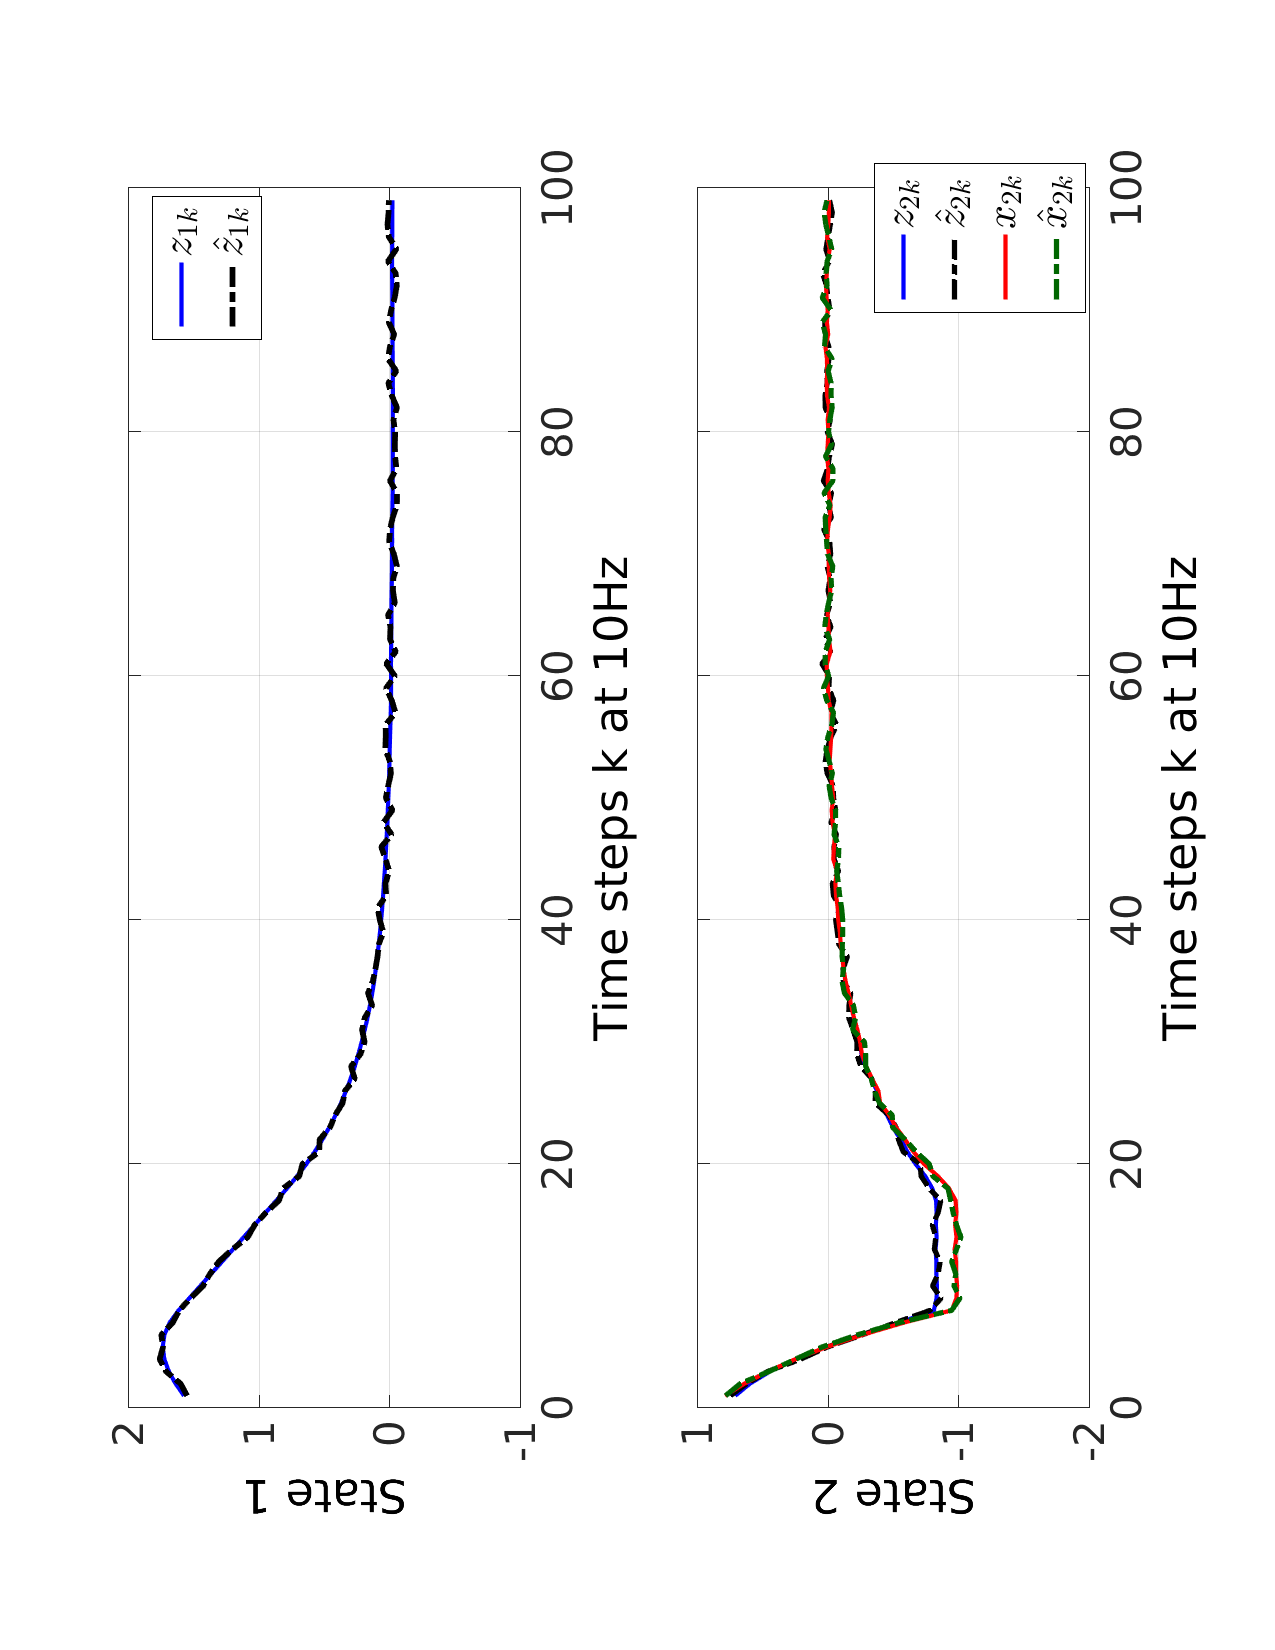
\includegraphics[angle=270,width=0.49\textwidth]{figs/AllStates_toy.pdf}
	\caption{The states and their estimates of the feedback linearized and non-linear running example. Recall that $z_1 = x_1$ therefore to reduce clutter, we only plot the first state only for the feedback linearized system. Color in online version.}
	\label{fig:AllStates_toy}
\end{figure}

For the running example of Eq. \ref{eq:toy_dynamics}, we discretize the feedback linearized system at 10Hz and formulate the controller with a horizon of $N=15$ steps. 
The cost function has parameters $Q=I$ and $R=10^{-2}$, and $W=[-10^{-2}, 10^{-2}]^2$.
The state trajectories (and estimates) for the nonlinear and linearized systems are shown in Fig. \ref{fig:AllStates_toy}.
Note that the states converge to the equilibrium 0. The input $u$ is shown in Fig. \ref{fig:input toy}, and it can be noted that $u_k \in U$ for all $k$.
%(and for the running example, $T$ preserves zero). 

\begin{figure}
	\centering	
	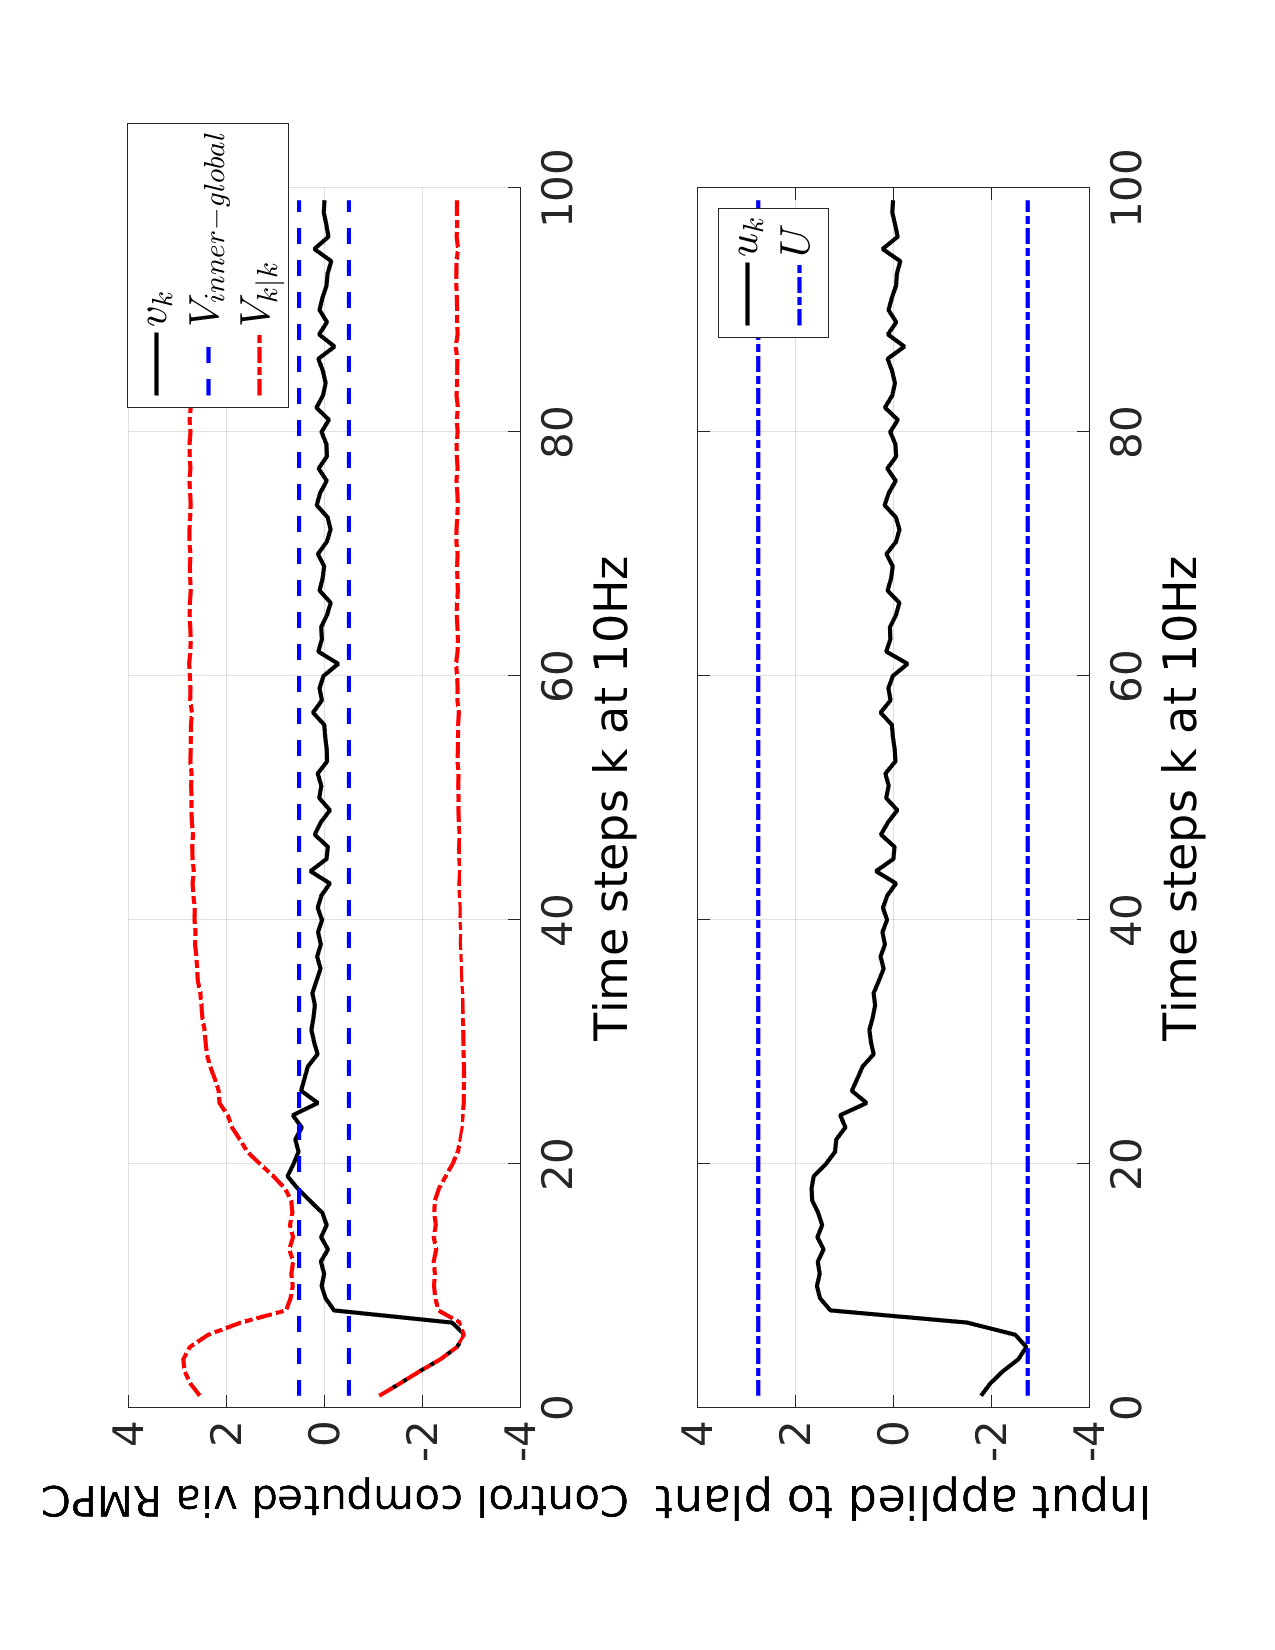
\includegraphics[angle=270,width=0.49\textwidth]{figs/u_and_v_toy.pdf}
	\caption{Inputs $v$ and $u$ and their bounds for the running example. Color in online version.}
	\label{fig:input toy}
\end{figure}


 %not in camera ready 

	


\end{document}
